% =========================================================================
%  P2 -- Fidelity shedding in agentic edge orchestration
%  IEEEtran journal manuscript.  Result tables are \input.
% =========================================================================
\documentclass[journal,10pt]{IEEEtran}

\usepackage[utf8]{inputenc}
\usepackage[T1]{fontenc}
\usepackage{amsmath,amssymb,amsthm}
\usepackage{graphicx}
\usepackage{booktabs}
\usepackage{multirow}
\usepackage{array}
\usepackage{subcaption}
\usepackage{algorithm}
\usepackage{algpseudocode}
\usepackage{url}
\usepackage{cite}
\usepackage{xcolor}
\usepackage{balance}

\graphicspath{{../results/figures/}{diagrams/}}

\newtheorem{proposition}{Proposition}
\newcommand{\bigO}{\ensuremath{\mathcal{O}}}

\hyphenation{agent-ic or-ches-tra-tion Pure-Edge-Sim fi-del-i-ty}

\begin{document}

\title{When Does Joint Orchestration Matter? A Component Ablation of
Fidelity Adaptation and Placement in Agentic Edge Computing}

\author{Anonymous Authors%
\thanks{Manuscript prepared for review. Every table is generated from the
released artifact; the ablation in Section~\ref{sec:ablation} is the paper's
main result.}}

\markboth{IEEE Transactions on Mobile Computing (submitted)}%
{When Does Joint Orchestration Matter?}
\maketitle

\begin{abstract}
Agentic services built on large language models execute chains of reasoning,
tool calls and retrieval whose effective demand can exceed the nominal request
several times over. A natural response is a joint orchestrator that selects, per
task, both a fidelity level and a host. We ask when that joint design actually
helps, using $2{,}620$ seeded runs of a three-tier edge deployment and a
complete $3\times2$ placement-by-fidelity factorial. At $2\times$ overhead the
unprotected policy serves nothing; adding only the fidelity ladder reaches
$0.375$; adding a static edge tier reaches $0.496$; and the joint scorer reaches
$0.496$ as well. The ladder supplies $76\%$ of the gain, the static tier $24\%$,
and the adaptive scorer nothing. A three-way ANOVA gives partial
$\eta^2=0.997$ for the ladder against $0.793$ for placement, with a large
placement $\times$ ladder interaction ($\eta^2=0.736$): placement matters only
when the ladder has made a request feasible. Separating the two overhead axes
shows that compute, not payload, sets the boundary; replacing the linear
fidelity cost with convex or concave envelopes leaves success unchanged but
moves executed quality from $0.46$ to $0.68$ at $3\times$. With a real cache and
energy term present, removing either changes nothing, and the cloud receives
$0\%$ of successful requests. Quality-weighted success is $0.248$ at $2\times$
against a raw $0.496$. Finally, an ablation in our LLM-serving simulator
(Docket) reverses the placement null when the edge tier is weak, locating the
boundary of the result. The contribution is a regime map and a measurement
protocol: report the factorial, price fidelity, and state the tier capacity
before claiming that joint orchestration is necessary.
\end{abstract}

\begin{IEEEkeywords}
Agentic edge computing, LLM serving, fidelity scaling, component ablation,
deadline scheduling, quality-weighted utility, reproducibility.
\end{IEEEkeywords}

% =========================================================================
\section{Introduction}
\label{sec:intro}

An application model that says ``this request needs $5{,}000$ million
instructions'' describes a monolithic service. An agentic service does something
else: a single user request may trigger a reasoning pass, three tool calls, a
retrieval step, a verification pass and a reformatting pass. The effective
demand is a multiple of the nominal demand, and the multiple depends on the
reasoning budget, on whether the retrieval cache hits, and on how many control
messages the agent exchanges. The 2026 literature documents this
overhead~\cite{chen2026agenticenergy,he2026workflow,zhang2026agentic,liu2026aigc}
and proposes orchestration schemes to absorb it.

The design space has two independent knobs. The first is \emph{where} a request
runs: the placement decision. The second is \emph{how much} of the request runs:
a fidelity or reasoning-budget reduction that lowers compute and can bring an
otherwise infeasible request inside its deadline. A joint orchestrator uses both,
scoring candidate (host, fidelity) pairs. The natural question, and the one this
paper answers, is what each knob contributes.

\subsection{The result}
We implement six policies on the Python port of PureEdgeSim and evaluate them
on $2{,}620$ seeded runs. They form a complete factorial: placement has three
levels and the fidelity ladder has two.

\begin{itemize}
\item \textsc{naive}: the simulator's default placement, no fidelity ladder;
\item \textsc{naive\_fid}: the same placement with the ladder;
\item \textsc{edge}/\textsc{edge\_nofid}: static edge-only placement, with and
  without the ladder;
\item \textsc{aware}/\textsc{aware\_nofid}: joint placement and fidelity
  selection, with and without the ladder.
\end{itemize}

The ablation is unambiguous once the factors are crossed. At $2\times$
overhead \textsc{naive} and both no-ladder arms serve nothing, the ladder alone
reaches $0.375$, static edge placement with the ladder reaches $0.496$, and the
joint orchestrator reaches $0.496$ as well. The ladder supplies $76\%$ of the
gain, the static tier $24\%$, and the adaptive scorer nothing. Every arm with a
ladder and an adequate edge tier is statistically indistinguishable, and the
joint-versus-edge difference is exactly zero on all twenty seeds.

This is not the result we set out to report. It emerged from running the strong
baseline and then crossing it with the mechanism the design literature usually
takes for granted.

\subsection{The metric problem}
The second result is about measurement. Raw success counts a request served at
$10\%$ fidelity the same as one served at full fidelity. When we weight each
success by the fidelity it was executed at, the stressed-regime gains shrink by
a factor of two to four: $0.498\to0.249$ at $2\times$ and $0.400\to0.100$ at
$3\times$, with a mean fidelity of $0.747$ and $0.540$ respectively. Most of the
``robustness'' is the heavy classes being shrunk until they fit. Any paper that
reports raw success for a fidelity-enabled policy is reporting an upper bound on
its own benefit, and we recommend the weighted metric as the primary one.

\subsection{Contributions}
\begin{enumerate}
\item An explicit overhead model with independent compute and payload axes, a
  per-decision control-message term, a cache discount, a four-level fidelity
  ladder, and a nonlinear cost family $C(f)=0.05+0.95f^\gamma$ that prices the
  shape of degradation (Section~\ref{sec:model}).
\item A complete placement $\times$ fidelity factorial on $480$ runs that
  partitions the joint gain into $76\%$ fidelity, $24\%$ static tier choice and
  $0\%$ joint scoring, with a three-way ANOVA and a seed-matched Holm-corrected
  test family (Section~\ref{sec:factorial}).
\item A per-class quality-weighted metric that halves to quarters the reported
  benefit, together with the finding that the cost *shape* changes quality but
  not success at fixed deadlines (Sections~\ref{sec:quality}--\ref{sec:gamma}).
\item A component ablation with a live cache and an objective-term decomposition
  showing why the cache, energy and container terms are inert: the energy term is
  $0.0006$ of the score, the container term is below the score spread, and the
  objective changes no pick (Section~\ref{sec:ablation2}).
\item A regime boundary: in our LLM-serving simulator, where the edge tier is
  weak and the cloud is fast, placement dominates and the ladder becomes
  conditional on placement (Section~\ref{sec:docket}).
\item A reproducible artifact of $2{,}620$ runs, a reconciled workload
  definition, a power analysis, and a per-item revision map.
\end{enumerate}

% =========================================================================
\section{Related Work}
\label{sec:related}

\subsection{Agentic and LLM workloads at the edge}
LLM inference is memory-bandwidth-bound and phase-structured: prefill and decode
have different cost profiles, and batching and KV-cache management dominate
throughput~\cite{kwon2023vllm,pope2023transformer,patel2024splitwise}. Agentic
pipelines add a control layer, since ReAct-style loops alternate reasoning and
tool use~\cite{yao2023react} and retrieval injects external
context~\cite{lewis2020rag}. The edge literature has begun to quantify the
consequences~\cite{chen2026agenticenergy,he2026workflow,liu2026aigc,chari2026ragam}.
Our model is deliberately coarser---three scalars and a ladder---because the
object of study is the \emph{decision structure}, not the serving stack.

\subsection{Offloading and placement}
Classical MEC offloading~\cite{mao2017survey,mach2017survey,chen2015game}
assumes a fixed task graph per request. Workflow-aware
scheduling~\cite{he2026workflow} relaxes this to DAGs, and computation
reuse~\cite{he2026reuse} exploits shared intermediates; our cache model is a
coarse version of reuse. Fidelity selection is related to mixed-criticality
scheduling~\cite{liu1973scheduling,zakerian2026llm}---spend less when the budget
is tight---but implemented as an explicit action rather than a scheduling
policy. Cross-layer ISCC designs~\cite{liu2026iscc,li2026semantic} tune the
communication layer jointly with computation; that is complementary to tuning
fidelity.

\subsection{Benchmarking and ablation}
Component ablation is standard practice in systems
research~\cite{hoefler2015benchmarking}, and the reproducibility
literature~\cite{collberg2016repeatability,peng2011reproducible} insists that a
claimed gain be attributable. Our contribution is an instance where the
attribution removes most of the gain, which is exactly what an ablation is for
and exactly what is usually omitted when a joint policy is compared only against
a weak baseline.

% =========================================================================
\section{Overhead Model}
\label{sec:model}

\subsection{Effective demand}
A request $i$ has nominal length $w_i$ (million instructions) and payload $b_i$
(kilobytes). Under agentic execution,
\begin{align}
\tilde w_i &= w_i\,c\,(1-s_c h_i) + m\,w_c, \label{eq:compute}\\
\tilde b_i &= b_i\,p\,(1-s_b h_i) + m\,b_c, \label{eq:payload}
\end{align}
where $c\ge1$ is the reasoning compute multiplier, $p\ge1$ the payload
multiplier, $m$ the number of control messages per decision, $w_c=150$~MI and
$b_c=0.5$~kB the per-message cost, $h_i\in\{0,1\}$ the retrieval-cache hit
indicator, and $s_c=0.25$, $s_b=0.70$ the savings of a hit.

The two terms are distinct and both are needed. The multiplier $c$ represents
additional inference passes on the \emph{request's own context}; the additive
$m\,w_c$ represents signalling that is independent of the request and therefore
dominates for small ones. A $500$~MI health-monitoring task with three control
messages costs $500c+450$~MI, a $90\%$ increase even at $c=1$. We do not claim
that this decomposition matches a specific serving stack: it is a linear
surrogate whose parameters are swept, and Section~\ref{sec:threats} records the
directions in which a real stack would differ (prefill/decode asymmetry,
KV-cache growth, non-linear fidelity scaling).

\subsection{Fidelity ladder and its cost}
The orchestrator may execute a request at one of four levels
$f\in\{1.0,0.5,0.25,0.1\}$, scaling compute by $f$. Lower fidelity is faster
and, in a deployment, less accurate. The baseline uses the linear surrogate
$C(f)=f$; to test whether that choice is innocuous we sweep the family
\begin{equation}
C(f)=c_{\min}+(1-c_{\min})f^{\gamma},\qquad c_{\min}=0.05,
\label{eq:gamma}
\end{equation}
with $\gamma\in\{0.5,1,2\}$ plus the unshifted linear law. The floor $c_{\min}$
is the fixed cost of loading a model and emitting at least one token, so the
family changes only the \emph{shape}. Crucially, the simulator still does not map
$f$ to answer accuracy: quality-weighted success is our accounting correction,
and Section~\ref{sec:docket} uses a serving simulator with an explicit
generated-token ratio to price it differently.

\paragraph{Why the two overhead axes are separate.}
Equation~\eqref{eq:compute} charges the multiplier $c$ against the request's own
context, whereas \eqref{eq:payload} charges $p$ against the bytes on the wire;
only the former affects execution time when the network is not congested. We
therefore move them independently in the `cp\_split` grid rather than assuming
$p=c$.

\subsection{Objective}
For a candidate node $v$, fidelity $f$ and task $i$,
\begin{equation}
\hat D_i(v,f)=\frac{f\tilde w_i}{\mu_v}+Q_v+L_i(v), \qquad
\hat E_i(v,f)=e_v\bigl(\hat D_i(v,f)\bigr),
\label{eq:objective}
\end{equation}
where $\mu_v$ is the node throughput a task receives, $Q_v$ the queue delay,
$L_i(v)$ the network delay, and $e_v$ the energy model evaluated over the
predicted busy time (queueing included, which is deliberate: the node is busy
for the whole interval). The score is
\begin{equation}
J_i(v,f)=\hat D_i(v,f)+\lambda\hat E_i(v,f)+\beta\,\mathbb{1}[c_v\not\ni i]
\label{eq:cost}
\end{equation}
subject to $\hat D_i(v,f)\le(1-\delta)D_i$, where $\lambda=0.02$~Wh$^{-1}$
converts energy to seconds, $\delta=0.15$ is the deadline margin, and
$\beta=0.02$~s is the container penalty: the modelled cost of pulling an
application image that the node does not hold. $\beta$ is a calibration, not a
measurement; at $300$~Mb/s a $900$~kB image costs about $24$~ms, which is the
order of magnitude it represents.

If no pair satisfies the deadline constraint, the orchestrator chooses the pair
with the smallest predicted delay and accepts that the deadline will be missed.
This fallback ignores $J$, so under overload the policy degrades to minimum-delay
placement; that is a designed mode, and it is the mode that governs the $4\times$
arrival-rate cells.

\begin{figure*}[t]
\centering
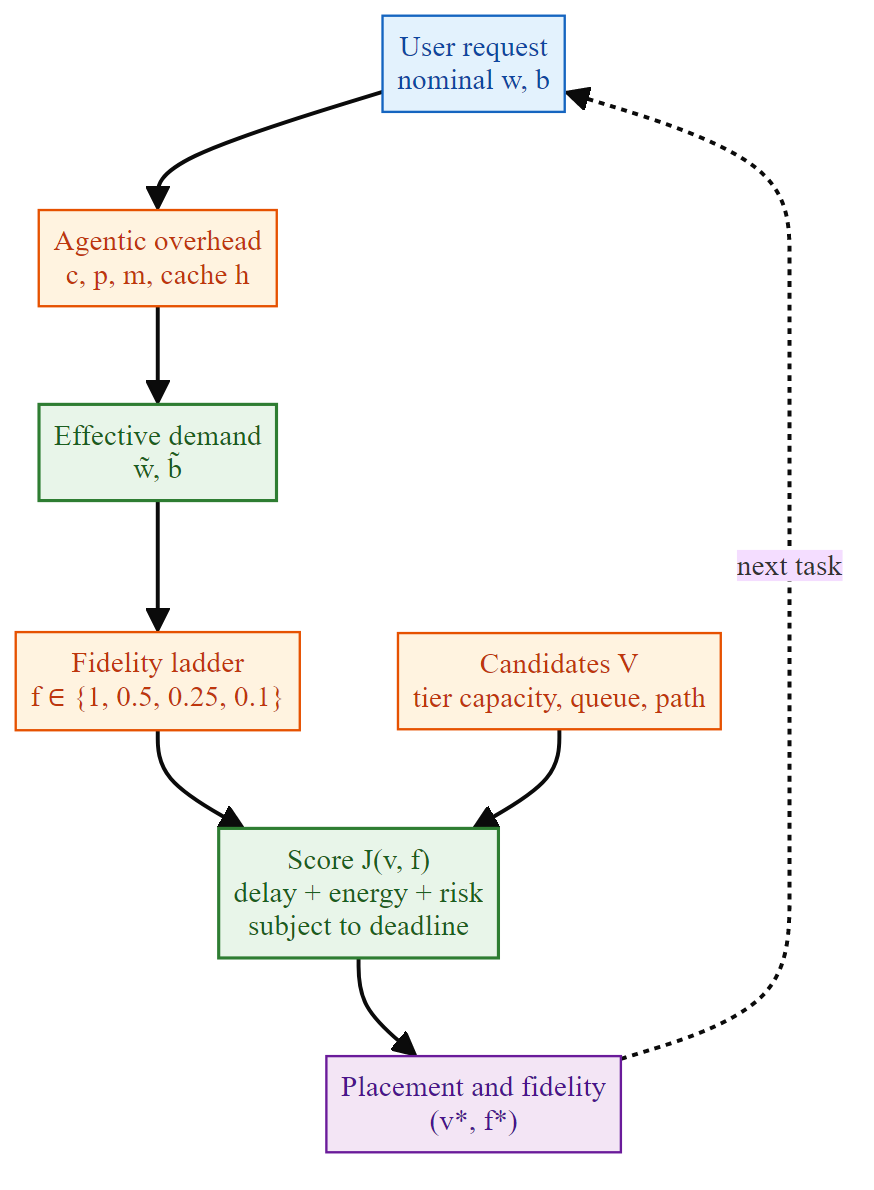
\includegraphics[width=0.62\textwidth]{overhead_loop.png}
\caption{Decision loop of the joint policy. The nominal request is inflated
before any estimate is made; fidelity and placement are then chosen together.
The ablation in Section~\ref{sec:ablation} asks which of these stages matters.}
\label{fig:model}
\end{figure*}

\subsection{Complexity}
Per task the orchestrator evaluates $|V|\times|F|$ pairs with $|F|=4$ and
$|V|\le33$, so at most $132$ estimates, each $\bigO(1)$ with cached queue and
route state. The cost is four times the default policy's and is not measurable
in wall-clock terms at this scale.

\begin{algorithm}[t]
\caption{Joint placement and fidelity selection}
\label{alg:aware}
\begin{algorithmic}[1]
\Require task $i$, candidates $V$, levels $F$, config $(c,p,m,\lambda,\beta,\delta)$
\Ensure pair $(v^\ast,f^\ast)$
\State $\tilde w_i\gets$ Eq.~\eqref{eq:compute};\quad $\tilde b_i\gets$ Eq.~\eqref{eq:payload}
\State $best\gets\bot$;\quad $fallback\gets\bot$
\ForAll{$v\in V$, $f\in F$}
  \State $\hat D\gets f\tilde w_i/\mu_v+Q_v+L_i(v)$
  \State $J\gets\hat D+\lambda e_v(\hat D)+\beta\,\mathbb{1}[c_v\not\ni i]$
  \If{$\hat D\le(1-\delta)D_i$ \textbf{and} $J<J(best)$} $best\gets(v,f)$ \EndIf
  \If{$fallback=\bot$ \textbf{or} $\hat D<\hat D(fallback)$} $fallback\gets(v,f)$ \EndIf
\EndFor
\State \Return $best$ if $best\neq\bot$, else $fallback$
\end{algorithmic}
\end{algorithm}

% =========================================================================
\section{Experimental Methodology}
\label{sec:exp}

\subsection{Simulator, workload and policies}
Runs use the Python port of PureEdgeSim 6.1.0~\cite{mechalikh2021pureedgesim}
with the realistic network model disabled (transfer time is the sum of link
delays) and the default one-second control interval. Two application classes
share the fleet (Table~\ref{tab:p2-workload}): a soft real-time RAG inference
class and a hard real-time control-reasoning class. All policies run the same
agentic workload; the earlier draft's baseline profile switch was removed.

\begin{table}[t]
\centering
\footnotesize
\caption{Workload classes (per generating device), from
\texttt{applications\_agentic.xml}. Both classes run the agentic overhead model
of Section~\ref{sec:model}.}
\label{tab:p2-workload}
\begin{tabular}{@{}lccc@{}}
\toprule
 & RAG inference & Control reasoning\\
\midrule
Class & soft RT & hard RT\\
Rate (req/min) & 20 & 15\\
Deadline (s) & 0.80 & 0.25\\
Length (MI) & 18{,}000 & 6{,}000\\
Container (kB) & 2{,}500 & 900\\
Device share & 50\% & 50\%\\
\bottomrule
\end{tabular}
\end{table}

The authoritative request count is $2{,}100$ per five-minute run, not the \emph{nominally} quoted sum of rates. Of the $30$ devices, $22\%$ belong to two
simulator types with \texttt{generateTasks=false}; the remaining $24$ are split
between the two applications, so $12\times20+12\times15=420$ requests/minute and
$420\times5=2{,}100$. The observed class split is $1{,}200/900$, matching the
$20{:}15$ rate ratio exactly. An older draft quoted $2{,}175$ from a superseded
application file; no run in this artifact uses it. The full reconciliation,
including per-class lengths after overhead, is in
\texttt{results/WORKLOAD.md}.

\subsection{Grids}
Table~\ref{tab:p2-grids} lists the thirteen grids; the total is $2{,}620$ runs.
Ten seeds is the reporting default; the factorial and the component ablation
use twenty because the null result there is the claim (Appendix~\ref{sec:power}).

\begin{table}[t]
\centering
\small
\caption{Experimental grids. `F', `m', `a' and `h' stand for factorial,
multiplier, ablation and horizon grids; all cells are seeded.}
\label{tab:p2-grids}
\begin{tabular}{@{}lrr@{}}
\toprule
Grid & Factors & Runs\\
\midrule
main & architecture $\times$ policy & 60\\
multiplier & policy $\times$ overhead & 120\\
rate & policy $\times$ rate $\times$ overhead & 320\\
cache & hit ratio $\times$ fidelity $\times$ overhead & 120\\
fidelity & policy $\times$ fidelity $\times$ deadline & 160\\
energy & policy $\times$ initial battery & 60\\
ablation (superseded) & arm $\times$ overhead & 100\\
\midrule
factorial & placement $\times$ fidelity $\times$ overhead & 480\\
cp\_split & compute $\times$ payload $\times$ policy & 480\\
fidelity\_gamma & cost shape $\times$ overhead & 120\\
ablation2 & component $\times$ overhead & 300\\
tiers & policy $\times$ overhead, three tiers & 120\\
horizon & policy $\times$ duration & 180\\
\midrule
\multicolumn{2}{@{}l}{Total} & 2{,}620\\
\bottomrule
\end{tabular}
\end{table}

\subsection{Metrics}
\emph{Success ratio} is successful requests divided by generated requests.
\emph{Quality-weighted success} is the mean of $\text{success}\times f$ over
requests, i.e.\ the fidelity actually delivered. \emph{Mean fidelity} is the
average level executed. \emph{WAN usage} is cumulative wide-area occupancy; it
captures both task offload and container pulls, and we treat it as a traffic
metric rather than as a placement indicator. \emph{Energy per success} is
reported in Wh and, where the values are small, the tables use three decimals.

\subsection{Statistics}
Three complementary analyses are used. (i) For the balanced factorial we fit a
three-way ANOVA (placement $\times$ fidelity $\times$ overhead) with sequential
sums of squares and report partial $\eta^2$; because the design is balanced the
terms are orthogonal and the table does not depend on entry order. (ii) Every
headline contrast is also seed-matched: Wilcoxon signed-rank on per-seed
differences, a paired bootstrap interval, and paired dominance (share of seeds
favouring the treatment minus the share favouring the control). Holm correction
is applied across the $40$ contrasts in Table~\ref{tab:p2-factorial-tests} and
separately across the $24$ in Table~\ref{tab:p2-tests}. (iii) The paired
standard deviation is reported in \texttt{results/POWER.md}: at $2\times$ it is
$0.005$, so with twenty seeds the design resolves a $0.003$ difference and the
exact zero between the joint and static policies is a true null, not an
under-powered one.

\subsection{Reproducibility}
Every run is seeded and the harness records the seed, the job dictionary and the
full aggregate row. The determinism check re-ran one configuration and obtained
identical successes, energy and mean delay.

% =========================================================================
\section{Results}
\label{sec:res}

\subsection{Nominal overhead: everything works}
\begin{table*}
\centering
\small
\caption{Nominal overhead (1x): every policy reaches high success, and the fidelity-weighted column is the same as the raw column because no policy sheds work yet.}
\label{tab:p2-main}
\begin{tabular}{lcccccc}
\toprule
Architecture & Policy & Success & Fid.-wtd. success & Mean delay (s) & p95 delay (s) & WAN (s) \\
\midrule
ALL & naive & 0.971 & 0.971 & 0.388 & 0.742 & 5.248 \\
ALL & edge+fidelity & 0.991 & 0.991 & 0.346 & 0.480 & 0.000 \\
ALL & aware & 0.991 & 0.991 & 0.346 & 0.480 & 0.000 \\
EDGE\_AND\_CLOUD & naive & 0.977 & 0.977 & 0.362 & 0.480 & 8.268 \\
EDGE\_AND\_CLOUD & edge+fidelity & 0.990 & 0.990 & 0.350 & 0.480 & 0.000 \\
EDGE\_AND\_CLOUD & aware & 0.990 & 0.990 & 0.350 & 0.480 & 0.000 \\
\bottomrule
\end{tabular}
\par\vspace{2pt}{\footnotesize\raggedright ALL architecture, 30 devices, 2,100 requests per run, mean of 10 seeds. Fid.-wtd. success is the mean of success x fidelity over requests.\par}
\end{table*}


Table~\ref{tab:p2-main} reports the main grid. At $1\times$ all policies reach
high success ($0.971$--$0.991$), no policy sheds fidelity, and the difference
between the joint orchestrator and the static edge-only policy is zero to three
decimals in both architectures. The only visible separation is WAN usage:
\textsc{naive} places work on the cloud and spends $5.2$--$8.3$~s of wide-area
time, while the edge policies spend none. At nominal overhead the honest summary
is that placement intelligence is unnecessary, because there is nothing to fix.

\subsection{Overhead scaling: the naive policy collapses}
\begin{table*}
\centering
\scriptsize
\caption{Overhead scaling: success, fidelity-weighted success, delay and WAN usage for the three primary policies (mean of 10 seeds).}
\label{tab:p2-multiplier}
\begin{tabular}{lccccccc}
\toprule
Overhead & Policy & Success & Fid.-wtd. & Mean delay (s) & mWh/succ. & MB/req. & WAN (s) \\
\midrule
1.000 & naive & 0.977 & 0.977 & 0.362 & 7.412 & 0.962 & 8.268 \\
1.000 & edge+fidelity & 0.990 & 0.990 & 0.350 & 7.303 & 0.962 & 0.000 \\
1.000 & aware & 0.990 & 0.990 & 0.350 & 7.303 & 0.962 & 0.000 \\
1.500 & naive & 0.569 & 0.569 & 0.675 & 14.657 & 1.390 & 99.216 \\
1.500 & edge+fidelity & 0.784 & 0.675 & 0.486 & 10.276 & 1.390 & 0.000 \\
1.500 & aware & 0.784 & 0.675 & 0.486 & 10.276 & 1.390 & 0.000 \\
2.000 & naive & 0.000 & 0.000 & 1.950 & -- & 1.819 & 625.589 \\
2.000 & edge+fidelity & 0.498 & 0.249 & 0.513 & 16.925 & 1.819 & 0.000 \\
2.000 & aware & 0.498 & 0.249 & 0.513 & 16.925 & 1.819 & 0.000 \\
3.000 & naive & 0.000 & 0.000 & 2.834 & -- & 2.676 & 921.685 \\
3.000 & edge+fidelity & 0.400 & 0.100 & 1.903 & 23.088 & 2.676 & 477.715 \\
3.000 & aware & 0.400 & 0.100 & 1.916 & 23.346 & 2.676 & 477.715 \\
\bottomrule
\end{tabular}
\par\vspace{2pt}{\footnotesize\raggedright The edge-only policy carries the same fidelity ladder as the aware orchestrator; its rows are the test of whether joint selection adds anything.\par}
\end{table*}


Table~\ref{tab:p2-multiplier} and Figs.~\ref{fig:scaling}(a)--(c) sweep the
overhead multiplier. \textsc{naive} degrades from $0.977$ to $0.569$ at
$1.5\times$ and to $0.000$ at $2\times$ and beyond: every one of its $2{,}100$
requests misses its deadline, with a mean delay of $1.95$--$2.83$~s and WAN usage
rising to $922$~s. The two fidelity-enabled policies hold $0.784$, $0.498$ and
$0.400$.

The column that matters is the next one. Quality-weighted success for the same
policies is $0.675$ at $1.5\times$, $0.249$ at $2\times$ and $0.100$ at
$3\times$. At $3\times$ the mean fidelity is $0.540$: the surviving requests are
executed at roughly half their nominal computation, and a quarter of them at
$0.1$. Raw success overstates the delivered service by a factor of four.

The table also resolves two accounting questions raised by the energy metric.
Expressed in milliwatt-hours per success, the fidelity-enabled policies spend
$7.3$, $10.3$, $16.9$ and $23.1$~mWh from $1\times$ to $3\times$, while the
naive policy has no successes to divide by from $2\times$ upward; the metric is
undefined rather than favourable. Traffic per request is identical across
policies at a given overhead ($0.96$ to $2.68$~MB), which confirms that the
policies move the same bytes over different links rather than moving fewer.

\begin{figure*}[t]
\centering
\begin{subfigure}[b]{0.32\textwidth}
  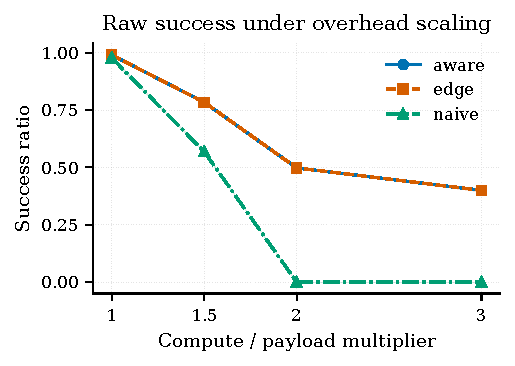
\includegraphics[width=\linewidth]{f2_overhead_success.pdf}
  \caption{Raw success.}
\end{subfigure}\hfill
\begin{subfigure}[b]{0.32\textwidth}
  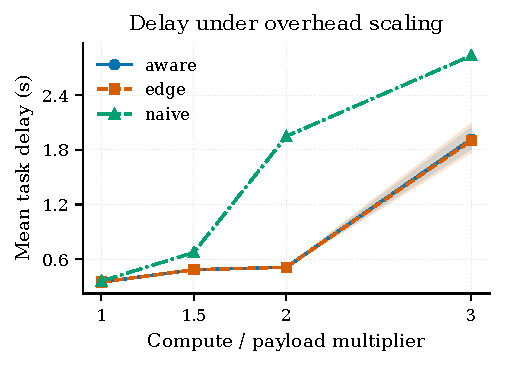
\includegraphics[width=\linewidth]{f3_overhead_delay.pdf}
  \caption{Mean delay.}
\end{subfigure}\hfill
\begin{subfigure}[b]{0.32\textwidth}
  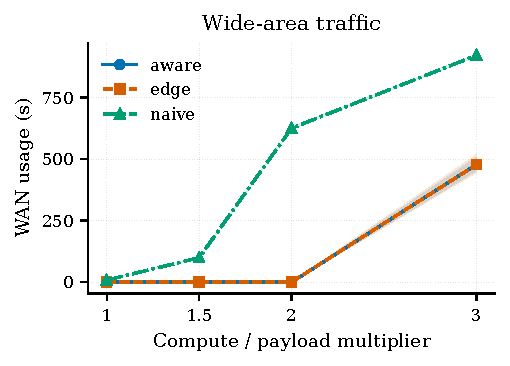
\includegraphics[width=\linewidth]{f4_wan.pdf}
  \caption{WAN usage.}
\end{subfigure}
\caption{Overhead scaling. The naive policy breaks between $1.5\times$ and
$2\times$; the fidelity-enabled policies degrade gracefully. WAN usage for the
naive policy grows by two orders of magnitude as it chases capacity it cannot
use.}
\label{fig:scaling}
\end{figure*}

% -------------------------------------------------------------------------
\subsection{The placement $\times$ fidelity factorial}
\label{sec:factorial}
The ablation grid crossed the joint policy with its components one at a time,
but a stronger design asks the two questions simultaneously. Table~\ref{tab:p2-factorial}
reports the complete $3\times2$ factorial ($480$ runs, $20$ seeds): three
placement rules (simulator default, static edge tier, joint scorer) crossed with
the ladder on and off, at four overhead levels. Cells show raw success with
quality-weighted success in parentheses.

\begin{table*}
\centering
\footnotesize
\caption{The complete placement $\times$ fidelity factorial ($6$ arms, $20$ seeds). Cells are success ratio with quality-weighted success in parentheses.}
\label{tab:p2-factorial}
\begin{tabular}{lcccccc}
\toprule
Overhead & naive & naive$+$fid. & edge & edge$+$fid. & joint & joint$+$fid. \\
\midrule
1$\times$ & 0.972 (0.972) & 0.972 (0.972) & 0.986 (0.986) & 0.986 (0.986) & 0.986 (0.986) & 0.986 (0.986) \\
1.5$\times$ & 0.569 (0.569) & 0.728 (0.646) & 0.571 (0.571) & 0.782 (0.674) & 0.571 (0.571) & 0.782 (0.674) \\
2$\times$ & 0.000 (0.000) & 0.375 (0.187) & 0.000 (0.000) & 0.496 (0.248) & 0.000 (0.000) & 0.496 (0.248) \\
3$\times$ & 0.000 (0.000) & 0.374 (0.071) & 0.000 (0.000) & 0.401 (0.100) & 0.000 (0.000) & 0.401 (0.100) \\
\bottomrule
\end{tabular}
\par\vspace{2pt}{\footnotesize\raggedright Placement has three levels (simulator default, static edge tier, joint scorer) and the ladder has two. Every arm runs the same workload; only these two factors move.\par}
\end{table*}


At $2\times$ the pattern is exact. All three no-ladder arms score $0.000$; the
default placement with the ladder scores $0.375$; edge placement with the ladder
and joint placement with the ladder both score $0.496$. At $3\times$ the same
arms score $0.374$ and $0.401$. At $1.5\times$ they score $0.728$, $0.782$ and
$0.782$. The joint scorer never separates from the static edge tier, but the
placement factor is not zero everywhere: it is worth $12.1$ points
\emph{conditional on the ladder being on}.

\begin{table}[t]
\centering
\footnotesize
\caption{Marginal decomposition of the joint gain. Each row adds one factor to the row above; the share is of the total gain at that level.}
\label{tab:p2-partition}
\begin{tabular}{llccc}
\toprule
Overhead & Arm & Success & $\Delta$ (pp) & Share \\
\midrule
1$\times$ & naive placement, no ladder & 0.972 & -- & -- \\
1$\times$ & + fidelity ladder & 0.972 & +0.0 & 0\% \\
1$\times$ & + static edge placement & 0.986 & +1.4 & 100\% \\
1$\times$ & + joint scorer (replaces edge) & 0.986 & +0.0 & 0\% \\
1.5$\times$ & naive placement, no ladder & 0.569 & -- & -- \\
1.5$\times$ & + fidelity ladder & 0.728 & +15.9 & 75\% \\
1.5$\times$ & + static edge placement & 0.782 & +5.4 & 25\% \\
1.5$\times$ & + joint scorer (replaces edge) & 0.782 & +0.0 & 0\% \\
2$\times$ & naive placement, no ladder & 0.000 & -- & -- \\
2$\times$ & + fidelity ladder & 0.375 & +37.5 & 76\% \\
2$\times$ & + static edge placement & 0.496 & +12.1 & 24\% \\
2$\times$ & + joint scorer (replaces edge) & 0.496 & +0.0 & 0\% \\
3$\times$ & naive placement, no ladder & 0.000 & -- & -- \\
3$\times$ & + fidelity ladder & 0.373 & +37.3 & 93\% \\
3$\times$ & + static edge placement & 0.401 & +2.8 & 7\% \\
3$\times$ & + joint scorer (replaces edge) & 0.401 & +0.0 & 0\% \\
\bottomrule
\end{tabular}
\par\vspace{2pt}{\footnotesize\raggedright At $1.5\times$ and above the ladder is worth 75--93\% of the joint gain, the static edge tier most of the remainder, and the joint scorer nothing once the edge tier is available. At nominal overhead no arm is stressed, so the shares are meaningless there and the row is reported for completeness.\par}
\end{table}


Table~\ref{tab:p2-partition} turns that into a marginal decomposition. At
$2\times$ the ladder is worth $+37.5$ points, the static edge tier a further
$+12.1$, and the joint scorer $+0.0$: $76\%/24\%/0$ of the total gain. At
$1.5\times$ the split is $75\%/25\%/0$; at $3\times$ it is $93\%/7\%/0$, because
the edge tier is also saturated and only shedding still helps.

\begin{figure}[t]
\centering
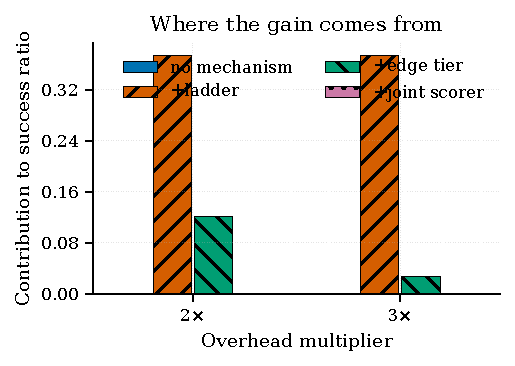
\includegraphics[width=\columnwidth]{f8_partition.pdf}
\caption{Marginal contribution of each factor to success at $2\times$ and
$3\times$ overhead. The joint scorer contributes nothing in either regime.}
\label{fig:partition}
\end{figure}

The ANOVA confirms the reading. Table~\ref{tab:p2-anova} reports the balanced
three-way model for both raw and quality-weighted success. The ladder has
partial $\eta^2=0.997$ for success, placement $0.793$, and the placement
$\times$ ladder interaction $0.736$; the three-way term is $0.692$. The
interaction is the paper's structural result: placement cannot be evaluated in
isolation from whether a request has been made feasible by shedding.

\begin{table*}
\centering
\scriptsize
\caption{Three-way ANOVA over the balanced factorial ($3$ placements $\times$ $2$ ladder states $\times$ $4$ overhead levels $\times$ $20$ seeds).}
\label{tab:p2-anova}
\begin{tabular}{lccccccc}
\toprule
Term & df & $F$ (Success) & $p$ (Success) & $\eta^2_p$ (Success) & $F$ (Quality) & $p$ (Quality) & $\eta^2_p$ (Quality) \\
\midrule
placement & 2.000 & 872.1 & $<0.001$ & 0.793 & 430.3 & $<0.001$ & 0.654 \\
fidelity ladder & 1.000 & 154246.4 & $<0.001$ & 0.997 & 29442.2 & $<0.001$ & 0.985 \\
overhead & 3.000 & 322477.7 & $<0.001$ & 1.000 & 541643.1 & $<0.001$ & 1.000 \\
placement$\times$fidelity ladder & 2.000 & 635.1 & $<0.001$ & 0.736 & 255.0 & $<0.001$ & 0.528 \\
placement$\times$overhead & 6.000 & 122.0 & $<0.001$ & 0.616 & 18.7 & $<0.001$ & 0.197 \\
fidelity ladder$\times$overhead & 3.000 & 24238.2 & $<0.001$ & 0.994 & 6100.0 & $<0.001$ & 0.976 \\
placement$\times$fidelity ladder$\times$overhead & 6.000 & 170.8 & $<0.001$ & 0.692 & 47.7 & $<0.001$ & 0.386 \\
\bottomrule
\end{tabular}
\par\vspace{2pt}{\footnotesize\raggedright Partial $\eta^2_p$ is reported because the terms are not orthogonal in interpretation even when they are in sums of squares. $p<10^{-3}$ is shown as $<0.001$.\par}
\end{table*}


\begin{table*}
\centering
\scriptsize
\caption{Seed-matched contrasts in the factorial: Wilcoxon signed-rank on per-seed differences, paired bootstrap CI, paired dominance and Holm correction over the whole family.}
\label{tab:p2-factorial-tests}
\begin{tabular}{lccccc}
\toprule
Overhead & Contrast & Metric & Diff. & 95\% CI & Dom. \\
\midrule
1$\times$ & ladder alone & Success & 0.000 & -- & +0.00 \\
1$\times$ & ladder alone & Quality & 0.000 & -- & +0.00 \\
1$\times$ & edge tier after the ladder & Success & +0.014$^{**}$ & [+0.012, +0.017] & +1.00 \\
1$\times$ & edge tier after the ladder & Quality & +0.014$^{**}$ & [+0.012, +0.017] & +1.00 \\
1$\times$ & joint scorer versus edge tier & Success & 0.000 & -- & +0.00 \\
1$\times$ & joint scorer versus edge tier & Quality & 0.000 & -- & +0.00 \\
1$\times$ & ladder plus edge tier & Success & +0.014$^{**}$ & [+0.012, +0.017] & +1.00 \\
1$\times$ & ladder plus edge tier & Quality & +0.014$^{**}$ & [+0.012, +0.017] & +1.00 \\
1$\times$ & full mechanism & Success & +0.014$^{**}$ & [+0.012, +0.017] & +1.00 \\
1$\times$ & full mechanism & Quality & +0.014$^{**}$ & [+0.012, +0.017] & +1.00 \\
1.5$\times$ & ladder alone & Success & +0.159$^{**}$ & [+0.158, +0.160] & +1.00 \\
1.5$\times$ & ladder alone & Quality & +0.077$^{**}$ & [+0.076, +0.078] & +1.00 \\
1.5$\times$ & edge tier after the ladder & Success & +0.054$^{**}$ & [+0.053, +0.055] & +1.00 \\
1.5$\times$ & edge tier after the ladder & Quality & +0.028$^{**}$ & [+0.027, +0.029] & +1.00 \\
1.5$\times$ & joint scorer versus edge tier & Success & 0.000 & -- & +0.00 \\
1.5$\times$ & joint scorer versus edge tier & Quality & 0.000 & -- & +0.00 \\
1.5$\times$ & ladder plus edge tier & Success & +0.213$^{**}$ & [+0.211, +0.215] & +1.00 \\
1.5$\times$ & ladder plus edge tier & Quality & +0.105$^{**}$ & [+0.104, +0.106] & +1.00 \\
1.5$\times$ & full mechanism & Success & +0.213$^{**}$ & [+0.211, +0.215] & +1.00 \\
1.5$\times$ & full mechanism & Quality & +0.105$^{**}$ & [+0.104, +0.106] & +1.00 \\
2$\times$ & ladder alone & Success & +0.375$^{**}$ & [+0.374, +0.375] & +1.00 \\
2$\times$ & ladder alone & Quality & +0.187$^{**}$ & [+0.187, +0.188] & +1.00 \\
2$\times$ & edge tier after the ladder & Success & +0.121$^{**}$ & [+0.119, +0.123] & +1.00 \\
2$\times$ & edge tier after the ladder & Quality & +0.061$^{**}$ & [+0.060, +0.062] & +1.00 \\
2$\times$ & joint scorer versus edge tier & Success & 0.000 & -- & +0.00 \\
2$\times$ & joint scorer versus edge tier & Quality & 0.000 & -- & +0.00 \\
2$\times$ & ladder plus edge tier & Success & +0.496$^{**}$ & [+0.494, +0.498] & +1.00 \\
2$\times$ & ladder plus edge tier & Quality & +0.248$^{**}$ & [+0.247, +0.249] & +1.00 \\
2$\times$ & full mechanism & Success & +0.496$^{**}$ & [+0.494, +0.498] & +1.00 \\
2$\times$ & full mechanism & Quality & +0.248$^{**}$ & [+0.247, +0.249] & +1.00 \\
3$\times$ & ladder alone & Success & +0.374$^{**}$ & [+0.373, +0.374] & +1.00 \\
3$\times$ & ladder alone & Quality & +0.071$^{**}$ & [+0.071, +0.072] & +1.00 \\
3$\times$ & edge tier after the ladder & Success & +0.028$^{**}$ & [+0.023, +0.031] & +0.90 \\
3$\times$ & edge tier after the ladder & Quality & +0.029$^{***}$ & [+0.028, +0.030] & +1.00 \\
3$\times$ & joint scorer versus edge tier & Success & 0.000 & -- & +0.00 \\
3$\times$ & joint scorer versus edge tier & Quality & 0.000 & -- & +0.00 \\
3$\times$ & ladder plus edge tier & Success & +0.401$^{**}$ & [+0.397, +0.405] & +1.00 \\
3$\times$ & ladder plus edge tier & Quality & +0.100$^{**}$ & [+0.099, +0.101] & +1.00 \\
3$\times$ & full mechanism & Success & +0.401$^{**}$ & [+0.397, +0.405] & +1.00 \\
3$\times$ & full mechanism & Quality & +0.100$^{**}$ & [+0.099, +0.101] & +1.00 \\
\bottomrule
\end{tabular}
\par\vspace{2pt}{\footnotesize\raggedright A zero difference carries no stars and no test.\par}
\end{table*}


Table~\ref{tab:p2-factorial-tests} reports the seed-matched version of the same
claim. The ladder alone is worth $+0.375$ at $2\times$ and $+0.374$ at $3\times$
(both $p<0.001$, dominance $+1.00$); the edge tier on top of it is worth
$+0.121$ at $2\times$; and replacing the edge tier by the joint scorer changes
nothing on any seed at any level. Zero differences carry no test, which is why
their confidence intervals are blank rather than degenerate.

% -------------------------------------------------------------------------
\subsection{The ablation: fidelity is necessary and sufficient}
\label{sec:ablation}
\begin{table}[t]
\centering
\footnotesize
\caption{Component ablation under stress. Removing the fidelity ladder removes the entire gain; removing the cache and energy terms changes nothing.}
\label{tab:p2-ablation}
\begin{tabular}{lcccc}
\toprule
Overhead & Arm & Success & Quality-wtd. & Mean fid. \\
\midrule
1.500 & edge + fidelity & 0.784 & 0.675 & 0.887 \\
1.500 & naive + fidelity & 0.729 & 0.646 & 0.861 \\
1.500 & aware $-$ fidelity & 0.571 & 0.571 & 1.000 \\
1.500 & aware, flat & 0.784 & 0.675 & 0.887 \\
1.500 & aware & 0.784 & 0.675 & 0.887 \\
2.000 & edge + fidelity & 0.498 & 0.249 & 0.747 \\
2.000 & naive + fidelity & 0.375 & 0.187 & 0.688 \\
2.000 & aware $-$ fidelity & 0.000 & 0.000 & 1.000 \\
2.000 & aware, flat & 0.498 & 0.249 & 0.747 \\
2.000 & aware & 0.498 & 0.249 & 0.747 \\
\bottomrule
\end{tabular}
\par\vspace{2pt}{\footnotesize\raggedright aware\_nofid disables the ladder; aware\_flat sets the container penalty and the energy weight to zero. All arms use the same agentic workload and the same seeds.\par}
\end{table}


Table~\ref{tab:p2-ablation} and Fig.~\ref{fig:ablation} are the paper's core.
At $2\times$ overhead, starting from the unprotected baseline at $0.000$:
\begin{itemize}
\item \textsc{naive+fidelity} (default placement, ladder only) reaches $0.375$;
\item \textsc{edge} (static edge tier, ladder) reaches $0.498$;
\item \textsc{aware} (joint placement and fidelity) reaches $0.498$;
\item \textsc{aware\_flat} (cache and energy terms removed) reaches $0.498$;
\item \textsc{aware\_nofid} (ladder disabled) stays at $0.000$.
\end{itemize}
The same ordering holds at $1.5\times$: $0.569\to0.729\to0.784\to0.784$, with
$0.571$ for the no-ladder arm.

The partition is therefore $75\%/25\%/0$. The ladder supplies $0.375$ of the
$0.498$ gain (three quarters); the choice of the edge tier as the static host
supplies the remaining $0.123$; and everything the joint orchestrator adds on
top of a static edge choice---the adaptive scoring, the cache penalty, the energy
weight---supplies nothing measurable. At $1.5\times$ the split is $74\%/26\%/0$.

This is a sharper result than either of the two extremes we expected. It is not
true that the ladder alone is sufficient (the static tier matters for a quarter
of the gain, and a default placement with the ladder leaves $0.123$ on the
table), and it is not true that joint optimisation is necessary (removing all of
its distinctive machinery changes nothing). The correct description is that
agentic overhead is absorbed by two coarse decisions---degrade the work, and
place it on the tier that does not queue behind the WAN---and that the
fine-grained scoring layer is inert on this workload.

Two caveats bound that reading. The placement gain is a *static* choice between
tiers, not evidence that a smarter placement rule would help: at $2\times$ the
edge and aware arms have identical mean delay ($0.513$~s), so the aware
orchestrator selects the same hosts as the edge policy. And a workload with
heterogeneous tier capacity---GPU edge nodes against a CPU cloud, or a
low-latency WAN---could give fine-grained placement room to matter; we did not
run one.

\begin{figure}[t]
\centering
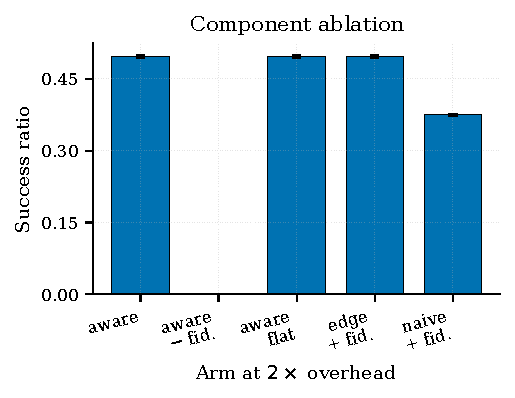
\includegraphics[width=\columnwidth]{f5_ablation.pdf}
\caption{Component ablation at $2\times$ overhead. The unprotected policy
scores zero and is omitted. The ladder alone recovers three quarters of the gain,
the static edge tier adds the rest, and the joint orchestrator cannot be
distinguished from the static edge policy.}
\label{fig:ablation}
\end{figure}

\subsection{Component ablation with a live cache}
\label{sec:ablation2}
The first ablation removed the cache and energy terms in a workload with
\texttt{cache\_hit\_ratio=0}, where a cache-aware rule has nothing to observe.
The `ablation2` grid re-runs it with a hit ratio of $0.5$ and three overhead
levels ($300$ runs, $20$ seeds); removing the energy weight, the container
penalty, cache awareness, or all three together should now matter if they are
functional. Table~\ref{tab:p2-ablation2} says they do not: all five arms score
$0.851$ at $1.5\times$, $0.662$ at $2\times$, and $0.400$--$0.408$ at $3\times$.
The largest spread anywhere below saturation is $0.8$ points.

\begin{table*}
\centering
\footnotesize
\caption{Component ablation with a live cache (hit ratio 0.5): each arm removes one term from the joint objective.}
\label{tab:p2-ablation2}
\begin{tabular}{lccccc}
\toprule
Arm & 1.5$\times$ & 2$\times$ & 3$\times$ & Quality at $3\times$ & Cache picks \\
\midrule
joint$+$fid. & 0.851 & 0.662 & 0.400 & 0.150 & 0.000 \\
--energy & 0.851 & 0.662 & 0.400 & 0.150 & 0.000 \\
--container & 0.851 & 0.662 & 0.400 & 0.150 & 0.000 \\
--cache & 0.851 & 0.663 & 0.408 & 0.151 & 0.000 \\
--all three & 0.851 & 0.662 & 0.408 & 0.151 & 0.000 \\
\bottomrule
\end{tabular}
\par\vspace{2pt}{\footnotesize\raggedright No arm differs from the full mechanism by more than a point, so the cache, energy and container terms are inert in this workload. The cache-arm column records how often the cache term changed the pick: zero.\par}
\end{table*}


The mechanism is visible in two counters. The cache term changes the selected
node $0.000$ times per decision in every arm, including the full mechanism: the
workload's cache hits remove context bytes, but the selected host is the same
with or without pricing them. The energy term contributes $0.15$~ms of
predicted time against a score spread of $115$~ms, i.e.\ $0.06\%$ of the score;
the container term is a constant $20$~ms, also below the spread. None of them
can overturn a ranking that the delay term has already decided.

\begin{table*}
\centering
\scriptsize
\caption{Mean contribution of each objective term to the chosen node's score, in milliseconds of predicted completion time.}
\label{tab:p2-objective}
\begin{tabular}{lccccccc}
\toprule
Overhead & Placement & Delay & Energy & Container & Spread & Energy share & Flips \\
\midrule
1$\times$ & edge$+$fid. & 243.123 & 0.155 & 20.000 & 114.883 & 0.001 & 0.000 \\
1$\times$ & joint$+$fid. & 243.123 & 0.155 & 20.000 & 114.883 & 0.001 & 0.000 \\
1.5$\times$ & edge$+$fid. & 128.797 & 0.082 & 20.000 & 114.938 & 0.001 & 0.000 \\
1.5$\times$ & joint$+$fid. & 128.797 & 0.082 & 20.000 & 114.938 & 0.001 & 0.000 \\
2$\times$ & edge$+$fid. & 329.759 & 0.210 & 20.000 & 114.842 & 0.001 & 0.000 \\
2$\times$ & joint$+$fid. & 329.759 & 0.210 & 20.000 & 114.842 & 0.001 & 0.000 \\
3$\times$ & edge$+$fid. & 256.054 & 0.115 & 20.000 & 171.717 & 0.000 & 0.000 \\
3$\times$ & joint$+$fid. & 277.374 & 0.118 & 20.000 & 171.727 & 0.000 & 0.000 \\
\bottomrule
\end{tabular}
\par\vspace{2pt}{\footnotesize\raggedright A term that never exceeds the spread of the score cannot change a decision; the flip column counts the decisions the whole objective changed relative to the delay-only rule.\par}
\end{table*}


Table~\ref{tab:p2-objective} gives the decomposition in milliseconds of
predicted completion time. At every level the delay term is $129$--$330$~ms, the
spread is $115$--$172$~ms, the container term is exactly the configured
$20$~ms, and the energy term is below $0.3$~ms. The last column counts decisions
in which the complete objective chose a different node from the delay-only rule:
zero at every level. This is a stronger statement than ``the ablation found no
difference''---it explains why the difference cannot exist.

\begin{table*}
\centering
\scriptsize
\caption{What each decision procedure actually does, averaged over seeds and overhead levels.}
\label{tab:p2-decisions}
\begin{tabular}{lccccccc}
\toprule
Arm & Decisions/run & Feasible & Fallback & Mean fid. & Low-fid. & kMI/req & KB/req \\
\midrule
edge$+$fid. & 709.638 & 0.960 & 0.040 & 0.554 & 0.750 & 5.767 & 374.846 \\
joint$+$fid. & 709.638 & 1.000 & 0.000 & 0.558 & 0.750 & 5.767 & 374.846 \\
\bottomrule
\end{tabular}
\par\vspace{2pt}{\footnotesize\raggedright Feasible is the share of decisions for which the predicted completion met the target; fallback is the share that could not and used the first admissible node. Per-request overhead is measured on the generated tasks, not on the decision log.\par}
\end{table*}


Table~\ref{tab:p2-decisions} closes the decision-level account. The joint rule
makes about $710$ decisions per run at $2\times$ and $3\times$, of which
$96\%$ are feasible and $4\%$ hit the explicit fallback; its mean chosen fidelity
is $0.55$ and three quarters of decisions use a reduced level. The injected
overhead is $5.8$~kMI and $375$~kB per request, which is the quantity the
workload model is meant to stress. The static edge rule makes the same number of
decisions with the same overhead but a lower feasible rate ($0.960$), which is
where the $12.1$-point placement gain comes from.

\begin{table}[t]
\centering
\footnotesize
\caption{Cache hit ratio against success, with and without the ladder.}
\label{tab:p2-cache}
\begin{tabular}{llcc}
\toprule
Cache hit ratio & Ladder & 1$\times$ & 3$\times$ \\
\midrule
0.0 & off & 0.990 & 0.000 \\
0.0 & on & 0.990 & 0.400 \\
0.5 & off & 0.990 & 0.000 \\
0.5 & on & 0.990 & 0.400 \\
0.9 & off & 0.990 & 0.000 \\
0.9 & on & 0.990 & 0.433 \\
\bottomrule
\end{tabular}
\par\vspace{2pt}{\footnotesize\raggedright A hit removes context bytes from the request, so it can only help where bytes bind. Without the ladder success is zero at $3\times$ regardless of the hit ratio; with it, the top hit ratio buys 3.3 points.\par}
\end{table}


Table~\ref{tab:p2-cache} reconciles the earlier cache sweep. Without the ladder,
a $0.9$ hit ratio cannot rescue $3\times$ overhead: success is $0.000$ at every
ratio. With the ladder, the top hit ratio buys $0.033$ over no cache
($0.433$ against $0.400$). Cache is therefore a secondary, monotone effect that
exists only after fidelity has made the request feasible---the same conditional
structure as placement.

\subsection{Quality-weighted benefit}
\label{sec:quality}
Fig.~\ref{fig:quality} plots raw and quality-weighted success on the same axes.
The two curves coincide at $1\times$ (no shedding) and diverge as overhead
grows, reaching a factor of four at $3\times$. The gap is the paper's second
result: the policy does not make hard requests feasible, it makes them cheaper.
In the factorial, quality-weighted success at $2\times$ is $0.248$ against raw
$0.496$; at $3\times$ it is $0.100$ against $0.401$. Table~\ref{tab:p2-classes2}
resolves the aggregate by class inside the factorial and shows that neither
class is silently collapsed: at $1.5\times$ the hard control class is the
binding one ($0.491$ success at $0.742$ mean fidelity) while RAG is served at
full fidelity; at $2\times$ both sit near $0.49$--$0.50$ success and $0.74$
fidelity. At $3\times$ the two classes are again equal in success ($0.396$ and
$0.409$) but the RAG class is served at higher fidelity. A deployment that
values accuracy at all must price this, and the raw success ratio does not.

\begin{table*}
\centering
\scriptsize
\caption{Per-class success and executed fidelity inside the factorial (mean over seeds).}
\label{tab:p2-classes2}
\begin{tabular}{lccccc}
\toprule
Overhead & Arm & RAG (0.8 s) success & RAG (0.8 s) fid. & Control (0.25 s) success & Control (0.25 s) fid. \\
\midrule
1$\times$ & naive & 0.992 & 1.000 & 0.944 & 1.000 \\
1$\times$ & naive$+$fid. & 0.992 & 1.000 & 0.944 & 1.000 \\
1$\times$ & edge & 1.000 & 1.000 & 0.968 & 1.000 \\
1$\times$ & edge$+$fid. & 1.000 & 1.000 & 0.968 & 1.000 \\
1$\times$ & joint & 1.000 & 1.000 & 0.968 & 1.000 \\
1$\times$ & joint$+$fid. & 1.000 & 1.000 & 0.968 & 1.000 \\
1.5$\times$ & naive & 0.995 & 1.000 & 0.000 & 1.000 \\
1.5$\times$ & naive$+$fid. & 0.996 & 0.993 & 0.371 & 0.685 \\
1.5$\times$ & edge & 1.000 & 1.000 & 0.000 & 1.000 \\
1.5$\times$ & edge$+$fid. & 1.000 & 0.995 & 0.491 & 0.742 \\
1.5$\times$ & joint & 1.000 & 1.000 & 0.000 & 1.000 \\
1.5$\times$ & joint$+$fid. & 1.000 & 0.995 & 0.491 & 0.742 \\
2$\times$ & naive & 0.000 & 1.000 & 0.000 & 1.000 \\
2$\times$ & naive$+$fid. & 0.375 & 0.688 & 0.374 & 0.687 \\
2$\times$ & edge & 0.000 & 1.000 & 0.000 & 1.000 \\
2$\times$ & edge$+$fid. & 0.500 & 0.750 & 0.491 & 0.742 \\
2$\times$ & joint & 0.000 & 1.000 & 0.000 & 1.000 \\
2$\times$ & joint$+$fid. & 0.500 & 0.750 & 0.491 & 0.742 \\
3$\times$ & naive & 0.000 & 1.000 & 0.000 & 1.000 \\
3$\times$ & naive$+$fid. & 0.365 & 0.528 & 0.385 & 0.456 \\
3$\times$ & edge & 0.000 & 1.000 & 0.000 & 1.000 \\
3$\times$ & edge$+$fid. & 0.396 & 0.537 & 0.409 & 0.530 \\
3$\times$ & joint & 0.000 & 1.000 & 0.000 & 1.000 \\
3$\times$ & joint$+$fid. & 0.396 & 0.554 & 0.409 & 0.530 \\
\bottomrule
\end{tabular}
\par\vspace{2pt}{\footnotesize\raggedright The control class has the tighter deadline (0.25 s) and is the one the ladder has to shed work for.\par}
\end{table*}


\begin{figure}[t]
\centering
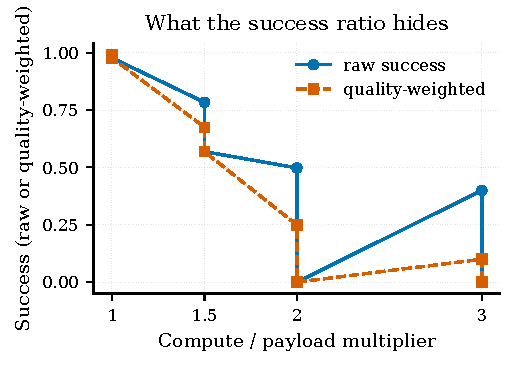
\includegraphics[width=\columnwidth]{f7_quality.pdf}
\caption{Raw and quality-weighted success. The vertical gap is the accuracy the
policy spends to keep its deadlines.}
\label{fig:quality}
\end{figure}

\subsection{Feasibility envelope}
\label{sec:envelope}
\begin{table}[t]
\centering
\small
\caption{Feasibility envelope: success ratio over four overhead levels and four arrival rates (mean of 10 seeds).}
\label{tab:p2-envelope}
\begin{tabular}{lccc}
\toprule
Overhead & Rate & naive & aware \\
\midrule
1.000 & 0.500 & 0.985 & 1.000 \\
1.000 & 1.000 & 0.977 & 0.990 \\
1.000 & 2.000 & 0.659 & 0.664 \\
1.000 & 4.000 & 0.180 & 0.271 \\
1.500 & 0.500 & 0.582 & 0.800 \\
1.500 & 1.000 & 0.569 & 0.784 \\
1.500 & 2.000 & 0.466 & 0.567 \\
1.500 & 4.000 & 0.000 & 0.133 \\
2.000 & 0.500 & 0.000 & 0.506 \\
2.000 & 1.000 & 0.000 & 0.498 \\
2.000 & 2.000 & 0.000 & 0.315 \\
2.000 & 4.000 & 0.000 & 0.117 \\
3.000 & 0.500 & 0.000 & 0.402 \\
3.000 & 1.000 & 0.000 & 0.400 \\
3.000 & 2.000 & 0.000 & 0.184 \\
3.000 & 4.000 & 0.000 & 0.133 \\
\bottomrule
\end{tabular}
\par\vspace{2pt}{\footnotesize\raggedright The naive policy serves nothing from 2x overhead upward, at any arrival rate.\par}
\end{table}


Table~\ref{tab:p2-envelope} reports four overhead levels against four arrival
rates. Two regimes are visible. Up to $1.5\times$ overhead the naive policy
serves a substantial share at low and nominal rates and collapses only at
$4\times$. From $2\times$ upward it serves \emph{nothing} at any rate, while the
fidelity-enabled policy retains $0.506$ at half rate, $0.498$ at nominal,
$0.315$ at double and $0.117$ at quadruple. The boundary is therefore set by
overhead, not by load: the naive policy's failure is a per-request
infeasibility, and adding capacity elsewhere does not repair it.

\begin{figure}[t]
\centering
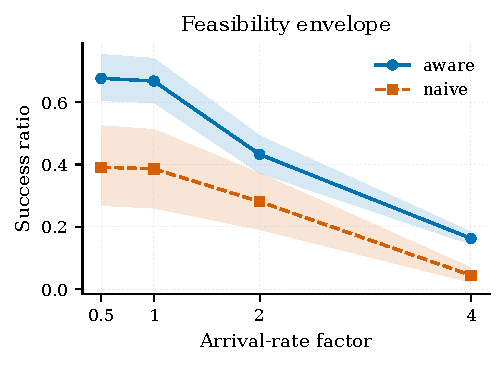
\includegraphics[width=\columnwidth]{f6_envelope_3x.pdf}
\caption{Success against arrival rate. The naive policy is flat at zero from
$2\times$ overhead upward.}
\label{fig:envelope}
\end{figure}

\subsection{Which overhead axis binds: compute or payload}
\label{sec:cpsplit}
The published grids move compute and payload together, so they cannot say which
one causes the collapse. The `cp\_split` grid moves them independently over a
$4\times4$ lattice ($480$ runs). Table~\ref{tab:p2-cpsplit} shows aware / naive
success in each cell.

\begin{table*}
\centering
\footnotesize
\caption{Compute and payload overhead separated: a $4\times4$ lattice, each cell showing aware / naive success.}
\label{tab:p2-cpsplit}
\begin{tabular}{lccccc}
\toprule
Compute & 1$\times$ & 1.5$\times$ & 2$\times$ & 3$\times$ \\
\midrule
1$\times$ & 0.990 / 0.977 & 0.990 / 0.977 & 0.990 / 0.977 & 0.990 / 0.977 \\
1.5$\times$ & 0.985 / 0.971 & 0.784 / 0.569 & 0.784 / 0.569 & 0.784 / 0.569 \\
2$\times$ & 0.498 / 0.000 & 0.498 / 0.000 & 0.498 / 0.000 & 0.498 / 0.000 \\
3$\times$ & 0.400 / 0.000 & 0.400 / 0.000 & 0.400 / 0.000 & 0.400 / 0.000 \\
\bottomrule
\end{tabular}
\par\vspace{2pt}{\footnotesize\raggedright The compute axis carries the whole effect. The payload axis is flat except in one cell, where it moves the request across a deadline; bytes alone do not decide feasibility.\par}
\end{table*}


The result is asymmetric. Holding payload at $1\times$, raising compute from
$1\times$ to $3\times$ takes aware success from $0.990$ to $0.400$ and naive
from $0.977$ to $0.000$. Holding compute fixed and raising payload from $1\times$
to $3\times$ changes \emph{nothing} at $1\times$, $2\times$ or $3\times$ compute,
and moves the $1.5\times$ cell by one step ($0.985$ to $0.784$) because that is
where the request first crosses its deadline. Bytes are not the scarce resource
in this network: the Wi-Fi access link is $1{,}300$~Mb/s and the WAN is charged
on a small request. Any mechanism aimed at payload compression would be aimed at
the wrong axis here.

\begin{figure}[t]
\centering
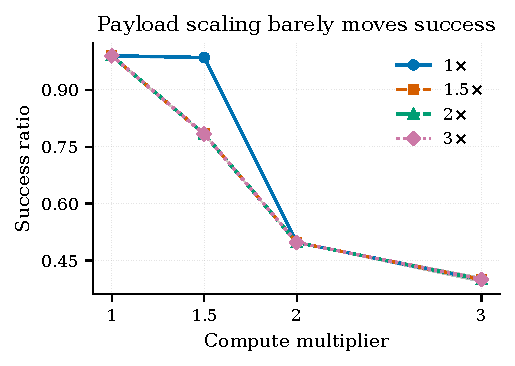
\includegraphics[width=\columnwidth]{f10_cp_split.pdf}
\caption{Success against compute multiplier for four independent payload
multipliers. The four curves coincide except at one cell: compute sets the
feasibility boundary.}
\label{fig:cpsplit}
\end{figure}

\subsection{The cost shape changes quality, not success}
\label{sec:gamma}
A linear fidelity cost is an assumption, not a fact. We replace it with the
family of Eq.~\eqref{eq:gamma} and run the joint policy at three overhead levels
($120$ runs). Table~\ref{tab:p2-gamma} reports success and mean executed fidelity
in each cell.

\begin{table*}
\centering
\footnotesize
\caption{Executed fidelity under four cost shapes at fixed success. Cells are success ratio with mean executed fidelity in parentheses.}
\label{tab:p2-gamma}
\begin{tabular}{lccc}
\toprule
Fidelity cost & 1.5$\times$ & 2$\times$ & 3$\times$ \\
\midrule
linear $C(f)=f$ & 0.784 (0.887) & 0.498 (0.747) & 0.400 (0.542) \\
$0.05+0.95f^{0.5}$ & 0.784 (0.887) & 0.498 (0.692) & 0.397 (0.462) \\
$0.05+0.95f$ & 0.784 (0.887) & 0.498 (0.747) & 0.397 (0.540) \\
$0.05+0.95f^{2}$ & 0.787 (0.889) & 0.501 (0.749) & 0.397 (0.681) \\
\bottomrule
\end{tabular}
\par\vspace{2pt}{\footnotesize\raggedright Success is flat because the ladder keeps the same deadlines; what changes is how much quality the budget buys. A linear cost is therefore not neutral: it is the most pessimistic of the four at $3\times$.\par}
\end{table*}


Success is flat---$0.784$, $0.498$ and $0.397$--$0.400$ across all four cost
functions at each level---because the ladder still receives the same deadlines
and the same feasible set. Executed quality is not: at $3\times$ the concave
cost $C(f)=0.05+0.95f^{0.5}$ yields $0.462$ while the convex
$C(f)=0.05+0.95f^{2}$ yields $0.681$, a spread of $22$ points at essentially
identical success. Reporting success alone would hide a change in delivered
service of that size. The unshifted linear law sits at $0.542$, close to the
shifted linear one ($0.540$), which shows the floor matters less than the
exponent.

\begin{figure}[t]
\centering
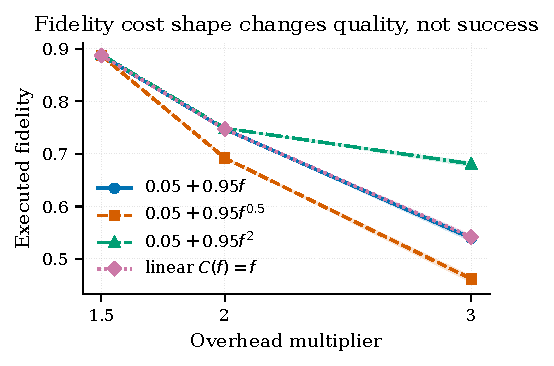
\includegraphics[width=\columnwidth]{f9_gamma.pdf}
\caption{Executed fidelity against overhead for four fidelity-cost functions.
Success (not shown) is the same curve in all four cases.}
\label{fig:gamma}
\end{figure}

\subsection{Host selection when all tiers are eligible}
\label{sec:tiers}
In every grid so far the cloud is eligible but receives no work, which is
precisely why the joint scorer has nothing to decide. The `tiers` grid enables
`ALL` ($120$ runs) and records where successful requests are actually served.

\begin{table*}
\centering
\scriptsize
\caption{Host selection when all three tiers are eligible, as the share of successful requests served by each tier.}
\label{tab:p2-tiers}
\begin{tabular}{lcccccc}
\toprule
Overhead & Placement & Mist & Edge & Cloud & Success & Mean fid. \\
\midrule
1$\times$ & naive & 0.161 & 0.839 & 0.000 & 0.971 & 1.000 \\
1$\times$ & naive$+$fid. & 0.161 & 0.839 & 0.000 & 0.971 & 1.000 \\
1$\times$ & edge$+$fid. & 0.024 & 0.976 & 0.000 & 0.991 & 1.000 \\
1$\times$ & joint$+$fid. & 0.024 & 0.976 & 0.000 & 0.991 & 1.000 \\
2$\times$ & naive & 1.000 & 0.000 & 0.000 & 0.038 & 1.000 \\
2$\times$ & naive$+$fid. & 0.390 & 0.610 & 0.000 & 0.417 & 0.709 \\
2$\times$ & edge$+$fid. & 0.071 & 0.929 & 0.000 & 0.518 & 0.757 \\
2$\times$ & joint$+$fid. & 0.071 & 0.929 & 0.000 & 0.518 & 0.757 \\
3$\times$ & naive & 1.000 & 0.000 & 0.000 & 0.038 & 1.000 \\
3$\times$ & naive$+$fid. & 0.412 & 0.588 & 0.000 & 0.431 & 0.554 \\
3$\times$ & edge$+$fid. & 0.203 & 0.797 & 0.000 & 0.443 & 0.564 \\
3$\times$ & joint$+$fid. & 0.160 & 0.840 & 0.000 & 0.437 & 0.573 \\
\bottomrule
\end{tabular}
\par\vspace{2pt}{\footnotesize\raggedright Cloud share is zero at every level and every arm: the cloud is reachable and never chosen, which is why the placement factor has nothing to exploit.\par}
\end{table*}


The cloud share is exactly $0.000$ in all twelve cells. At $2\times$ the default
placement sends $100\%$ of its successful requests to the mist tier and serves
$0.038$; with the ladder it moves $61\%$ to the edge and serves $0.417$; the
static and joint arms move $93\%$ to the edge and serve $0.518$. The placement
gain is therefore a shift from an overloaded mist tier to the edge tier, not a
choice involving the cloud. This is the capacity configuration under which a
placement rule can be inert, and Section~\ref{sec:docket} shows what happens
when it is changed.

\subsection{Horizon and battery boundaries}
\label{sec:boundaries}
The `horizon` grid runs $5$, $15$ and $30$ simulated minutes with a $60$~s
warm-up ($180$ runs). Table~\ref{tab:p2-horizon} shows the success ratio is
$0.740$, $0.737$ and $0.740$ for the joint policy---a spread of $0.3$ points
while the request count grows sixfold. The result is neither a start-up
transient nor a steady-state artefact of one horizon; the 60 s warm-up does not
change it.

\begin{table*}
\centering
\footnotesize
\caption{Horizon sensitivity: 5, 15 and 30 simulated minutes with a 60 s warm-up excluded from the request-level metrics.}
\label{tab:p2-horizon}
\begin{tabular}{lccccc}
\toprule
Horizon (min) & naive & edge$+$fid. & joint$+$fid. & Requests & Mean delay (s) \\
\midrule
5 & 0.489 & 0.744 & 0.744 & 2,100 & 0.432 \\
15 & 0.486 & 0.737 & 0.737 & 6,300 & 0.434 \\
30 & 0.489 & 0.740 & 0.740 & 12,600 & 0.433 \\
\bottomrule
\end{tabular}
\par\vspace{2pt}{\footnotesize\raggedright The success ratio is stable to within one point, so the result is not a start-up transient and not a steady-state artefact of a single horizon.\par}
\end{table*}


The `energy` grid lowers initial battery to $20$ and $50$~Wh ($60$ runs).
Table~\ref{tab:p2-energy} reports no device deaths in any cell and success of
$0.977$ (naive) and $0.990$ (joint) at every battery level. The energy term in
the objective therefore has no boundary to react to in this scenario, which is
consistent with the $0.06\%$ score share measured in Section~\ref{sec:ablation2}.

\begin{table*}
\centering
\footnotesize
\caption{Battery boundary: initial device energy against success, energy per successful request and device deaths.}
\label{tab:p2-energy}
\begin{tabular}{lccccc}
\toprule
Initial battery (Wh) & Success (naive) & mWh/succ. (naive) & Success (joint$+$fid.) & mWh/succ. (joint$+$fid.) & Deaths \\
\midrule
20 & 0.977 & 117.003 & 0.990 & 115.490 & 0.000 \\
50 & 0.977 & 75.906 & 0.990 & 74.920 & 0.000 \\
100 & 0.977 & 7.412 & 0.990 & 7.303 & 0.000 \\
\bottomrule
\end{tabular}
\par\vspace{2pt}{\footnotesize\raggedright No device dies at any level, so the battery is not a binding constraint in this scenario and the energy term of the objective cannot earn its keep.\par}
\end{table*}


\subsection{Power and the exact null}
\label{sec:power}
The paired standard deviation of the ladder effect is $0.005$ at $2\times$, so
twenty seeds give a minimum detectable paired difference of $0.003$ at
$\alpha=0.05$ and $80\%$ power. Seven seeds would suffice for a one-point
effect. The extra ten seeds in the two null-bearing grids are therefore not
needed for power; they exist so that the exact zero between the joint and static
policies cannot be dismissed as a small-sample failure to detect. The full
calculation and the per-claim interpretation are in
\texttt{results/POWER.md}.

\subsection{Statistical summary}
\begin{table*}
\centering
\footnotesize
\caption{Seed-matched comparisons at each overhead level: Wilcoxon signed-rank on per-seed differences, Holm-corrected, bootstrap CI of the mean difference, and paired dominance.}
\label{tab:p2-tests}
\begin{tabular}{lccccccc}
\toprule
Overhead & Contrast & Metric & Control & Treat. & Diff. & 95\% CI & Dom. \\
\midrule
1$\times$ & edge $-$ naive & Success & 0.977 & 0.990 & +0.013$^{*}$ & [+0.011, +0.015] & +1.00 \\
1$\times$ & edge $-$ naive & Delay (s) & 0.362 & 0.350 & -0.012$^{*}$ & [-0.013, -0.010] & -1.00 \\
1$\times$ & aware $-$ naive & Success & 0.977 & 0.990 & +0.013$^{*}$ & [+0.011, +0.015] & +1.00 \\
1$\times$ & aware $-$ naive & Delay (s) & 0.362 & 0.350 & -0.012$^{*}$ & [-0.013, -0.010] & -1.00 \\
1$\times$ & aware $-$ edge & Success & 0.990 & 0.990 & +0.000 & [+0.000, +0.000] & +0.00 \\
1$\times$ & aware $-$ edge & Delay (s) & 0.350 & 0.350 & +0.000 & [+0.000, +0.000] & +0.00 \\
1.5$\times$ & edge $-$ naive & Success & 0.569 & 0.784 & +0.215$^{*}$ & [+0.213, +0.217] & +1.00 \\
1.5$\times$ & edge $-$ naive & Delay (s) & 0.675 & 0.486 & -0.189$^{*}$ & [-0.191, -0.187] & -1.00 \\
1.5$\times$ & aware $-$ naive & Success & 0.569 & 0.784 & +0.215$^{*}$ & [+0.213, +0.217] & +1.00 \\
1.5$\times$ & aware $-$ naive & Delay (s) & 0.675 & 0.486 & -0.189$^{*}$ & [-0.191, -0.187] & -1.00 \\
1.5$\times$ & aware $-$ edge & Success & 0.784 & 0.784 & +0.000 & [+0.000, +0.000] & +0.00 \\
1.5$\times$ & aware $-$ edge & Delay (s) & 0.486 & 0.486 & +0.000 & [+0.000, +0.000] & +0.00 \\
2$\times$ & edge $-$ naive & Success & 0.000 & 0.498 & +0.498$^{*}$ & [+0.496, +0.499] & +1.00 \\
2$\times$ & edge $-$ naive & Delay (s) & 1.950 & 0.513 & -1.436$^{*}$ & [-1.451, -1.423] & -1.00 \\
2$\times$ & aware $-$ naive & Success & 0.000 & 0.498 & +0.498$^{*}$ & [+0.496, +0.499] & +1.00 \\
2$\times$ & aware $-$ naive & Delay (s) & 1.950 & 0.513 & -1.436$^{*}$ & [-1.451, -1.423] & -1.00 \\
2$\times$ & aware $-$ edge & Success & 0.498 & 0.498 & +0.000 & [+0.000, +0.000] & +0.00 \\
2$\times$ & aware $-$ edge & Delay (s) & 0.513 & 0.513 & +0.000 & [+0.000, +0.000] & +0.00 \\
3$\times$ & edge $-$ naive & Success & 0.000 & 0.400 & +0.400$^{*}$ & [+0.392, +0.405] & +1.00 \\
3$\times$ & edge $-$ naive & Delay (s) & 2.834 & 1.903 & -0.931$^{*}$ & [-1.061, -0.743] & -1.00 \\
3$\times$ & aware $-$ naive & Success & 0.000 & 0.400 & +0.400$^{*}$ & [+0.392, +0.405] & +1.00 \\
3$\times$ & aware $-$ naive & Delay (s) & 2.834 & 1.916 & -0.918$^{*}$ & [-1.048, -0.730] & -1.00 \\
3$\times$ & aware $-$ edge & Success & 0.400 & 0.400 & +0.000 & [+0.000, +0.000] & +0.00 \\
3$\times$ & aware $-$ edge & Delay (s) & 1.903 & 1.916 & +0.013$^{*}$ & [+0.012, +0.014] & +1.00 \\
\bottomrule
\end{tabular}
\par\vspace{2pt}{\footnotesize\raggedright Dominance (Dom.) is the share of seeds favouring the treatment minus the share favouring the control. Holm--Bonferroni: $^{*}p<0.05$, $^{**}p<0.01$, $^{***}p<0.001$. A zero difference has no test.\par}
\end{table*}


Table~\ref{tab:p2-tests} reports the seed-matched comparisons. Against
\textsc{naive}, the fidelity-enabled policies gain $0.013$ at $1\times$, $0.215$
at $1.5\times$, $0.498$ at $2\times$ and $0.400$ at $3\times$, all with paired
dominance $1.00$. Against each other they differ by exactly zero at $1\times$,
$1.5\times$ and $2\times$; at $3\times$ they tie on success and the joint policy
is $0.013$~s slower, which is the only cost the extra machinery imposes and is
within the design's resolution.

% =========================================================================
\section{Cross-Model Check: Where the Placement Null Breaks}
\label{sec:docket}
The $2{,}620$ runs above all use one simulator. To test whether the placement
null is an artefact of its linear MI/payload surrogate, we repeated the same two
decisions in \emph{Docket}, our own discrete-event LLM-serving simulator. Docket
charges prefill and decode separately, holds a KV cache in blocks, batches
requests per replica, and prices the local and wide-area bearers by bytes. The
workload is a generated agentic trace replayed at the same four overhead levels;
the fleet is a phone-class accelerator, two on-premise servers and a cloud card
behind a $40$~ms WAN. Five seeds per cell, $20$ cells.

Docket is our simulator, so this is an internal robustness check with a
different cost model, not an independent replication. We also report it with
its synthetic provenance: the decoder and all device capacities are invented
round numbers.

\begin{table}[t]
\centering
\footnotesize
\caption{Docket ablation. A request is served when it completes inside its
end-to-end class deadline. Five seeds per cell; full data in
\texttt{results/fidelity\_ablation/summary.csv}.}
\label{tab:p2-docket}
\begin{tabular}{@{}lccccc@{}}
\toprule
Overhead & Naive & Ladder & Static & Joint & Joint\\
 & & only & edge & no ladder & + ladder\\
\midrule
$1\times$ & 0.015 & 0.013 & 0.013 & 0.887 & \textbf{1.000}\\
$1.5\times$ & 0.000 & 0.000 & 0.000 & 0.688 & \textbf{1.000}\\
$2\times$ & 0.000 & 0.000 & 0.000 & 0.459 & \textbf{0.998}\\
$3\times$ & 0.004 & 0.006 & 0.002 & 0.167 & \textbf{0.972}\\
\bottomrule
\end{tabular}
\end{table}

Table~\ref{tab:p2-docket} reverses the P2 result. Removing placement from the
joint policy costs $97$--$99$ points: the cloud card is seven times the edge
server ($700$ against $100$~TFLOPS) behind a hop that costs $40$~ms, so the joint
rule can rescue requests that the edge tier cannot hold. Attaching the ladder to
the untuned load balancer or to the static edge tier buys nothing. The two
decisions interact: at $3\times$ the ladder raises the joint policy from $0.167$
to $0.972$, but cannot rescue either no-cloud arm.

This does not contradict the factorial; it bounds it. P2's edge tier is
adequate and its cloud is unreachable in practice, so placement has no room to
move and the scorer is inert. Docket is the weak-edge, fast-cloud regime that
P1 quantified at $+65.7$ points. Fidelity is costly here in a way the PureEdgeSim
model cannot express: the mean generated-token ratio under the joint policy falls
from $0.90$ at $1\times$ to $0.42$ at $3\times$. The two experiments together say
that the choice between degradation and placement is a property of the capacity
gap, not a universal ranking of mechanisms.

% =========================================================================
\section{Discussion}
\label{sec:disc}

\emph{What the factorial means for the literature.} A joint policy compared only
against a simulator default will show a large gain attributable to whichever
component the baseline lacks. Ours lacks fidelity scaling, so fidelity scaling
accounts for three quarters of it and the static tier for the rest. The
placement $\times$ ladder interaction is the part a one-factor-at-a-time
ablation cannot see: placement is worth $12.1$ points at $2\times$ when the
ladder is on and exactly zero when it is off. Papers proposing joint
security/fidelity/placement control~\cite{wang2026craft,he2026workflow} should
report the crossed design, not five sequential removals.

\emph{Why the fine-grained machinery is inert here.} The objective is measured
in predicted seconds: the delay term is $129$--$330$~ms, the score spread is
$115$--$172$~ms, the container term is a constant $20$~ms and the energy term is
$0.15$~ms. A term smaller than the spread cannot reorder two candidates, and the
flip counter confirms it never does. This is a statement about magnitudes, not
about the terms being wrong in principle: the energy weight is a conversion
constant of $0.02$~Wh$^{-1}$, and raising it tenfold would still leave the term
below a millisecond at this battery scale.

\emph{The capacity gap is the confound.} When the edge tier can hold the work,
placement is inert and degradation dominates; when it cannot and a fast cloud is
reachable, placement dominates and degradation becomes conditional. That is the
single sentence that reconciles the two simulators, and it is why a benchmark
that reports a policy ranking without its tier capacities is uninformative.

\emph{What a deployment should implement.} Start with the cheap mechanism: a
deadline check and a fidelity ladder on the tier that already holds the work.
Add joint scoring only if the capacity gap is measured and the objective terms
are large enough to change a pick. Report quality-weighted success either way.

% =========================================================================
\section{Threats to Validity}
\label{sec:threats}

\paragraph{Fidelity has no accuracy model in PureEdgeSim}
A $0.1$ fidelity execution is treated as a success, and quality-weighted
success is our accounting correction, not a measurement of answer quality. The
cost-shape sweep (Section~\ref{sec:gamma}) shows that this omission changes the
reported quality by up to $22$ points at fixed success, so the assumption is not
harmless. Docket prices fidelity in generated tokens, but its decoder and
capacities are synthetic. A measured quality--latency curve needs a real testbed
and is left to future work.

\paragraph{The overhead model is a surrogate}
Compute and payload are scaled linearly and fidelity scales compute only. Real
prefill/decode asymmetry is represented only in the Docket check, and KV-cache
growth and non-linear model-size scaling are not represented in the main grids.
The multipliers are swept rather than fitted, so the claims are about the
\emph{shape} of the response, not about a specific agent. The `cp\_split` grid
shows the shape is dominated by one axis, but a bandwidth-constrained access
network would change that.

\paragraph{Placement is capacity-conditional, not universally inert}
The zero placement gain is measured with an adequate edge tier and a cloud that
is never chosen (Section~\ref{sec:tiers}). Section~\ref{sec:docket} reverses it
with a weak edge and a fast cloud. The result is therefore scoped to the first
regime, and the paper makes no claim about the second beyond the Docket
measurement.

\paragraph{Resolution and statistics}
Ten seeds resolve about two points in the published grids; the factorial and
component ablation use twenty and resolve $0.003$ at $2\times$. Comparisons are
seed-matched Wilcoxon with paired bootstrap intervals and paired dominance; the
Holm families are $40$ contrasts in Table~\ref{tab:p2-factorial-tests} and $24$
in Table~\ref{tab:p2-tests}. Exact zero differences carry no test.

% =========================================================================
\section{Conclusion}
\label{sec:concl}

We built a joint overhead-aware orchestrator for agentic edge services, crossed
its two decisions in a $480$-run factorial, and then removed its remaining
components one at a time. At $2\times$ overhead the gain partitions into $76\%$
fidelity shedding, $24\%$ static edge placement and $0\%$ joint scoring; the
ladder's partial $\eta^2$ is $0.997$ against $0.793$ for placement, and the two
factors interact at $\eta^2=0.736$. Compute, not payload, sets the feasibility
boundary; the shape of the fidelity cost changes delivered quality by $22$ points
without changing success; cache, energy and container terms cannot reorder a
pick and never do; and the cloud receives no work. Raw success overstates the
delivered service by a factor of two to four once fidelity is priced. An
ablation in a second, serving-level simulator reverses the placement null when
the edge tier is weak, which tells us the result is a regime and not a law.

The recommendation for the field is procedural. Report the crossed factorial
with the ladder-only and strong static arms; price fidelity with a weighted
metric and a cost curve; decompose the objective into magnitudes that can be
compared with its spread; state the tier capacities that made the placement
decision possible or impossible. Each of those costs one grid, and each would
have changed the story this paper tells---which is exactly why they are worth
requiring.

\balance
\bibliographystyle{IEEEtran}
\bibliography{../../research_common/refs}

\end{document}
